\subsection{Beleuchtungstest}
\label{chap:LichtTest}
%\begin{tabular}{p{3.6cm}p{9.4cm}}
%\rule{0pt}{11pt}\textit{Typ}              & 4 Bauscheinwerfer \\ 
%\rule{0pt}{11pt}\textit{Datum}:           & 04.12.2014   \\
%\rule{0pt}{11pt}\textit{Ort}:             & originales Spielfeld \\
%\rule{0pt}{11pt}\textit{Tester}:          & Gruppe 32 \\
%\rule{0pt}{11pt}\textit{Ziel des Testes}: & Den Schattenwurf, welcher von der Beleuchtung verursacht wird auf der Stützwand hinter dem Kübel zu rekonstruieren. \\
%\rule{0pt}{11pt}\textit{Fazit / Verbesserungs-\newline vorschlag}: & 
%Der Schattenwurf kann vernachlässigt werden. Die Bilderkennung wird durch den Schatten nicht gestört. 
%\end{tabular}

\begin{tabular}{p{3.6cm}p{\textwidth-3.6cm-0.7cm}}
	\rule{0pt}{11pt}\textit{Typ}              & Lichttest  \\ 
	\rule{0pt}{11pt}\textit{Datum}:           & 04.12.2014   \\
	\rule{0pt}{11pt}\textit{Ort}:             & Teaminseln, Trakt 3 HSLU \\
	\rule{0pt}{11pt}\textit{Tester}:          & Thomas, Pascal, Livio, Matteo, Niklaus\\
	\rule{0pt}{11pt}\textit{Ziel des Testes}: & Es soll festgestellt werden, ob der entwickelte 
	Algorithmus zur Korberkennung bei Verwendung von starken Scheinwerfern funktioniert. Besonderes Augenmerk liegt auf dem Schattenwurf auf der Rückwand und die Belichtung des Korbes selbst. \\
	\rule{0pt}{11pt}\textit{Aufbau / Ablauf}: & Das Modellspielfeld wurde mit zwei ??? Watt 
	Scheinwerfern ausgeleuchtet und anschliessend mit mehreren Smartphones (LG Nexus, HTC One 
	und Nokia Lumia) abfotografiert. Die Resultate wurden dem entwickelten Prototypen zur Auswertung übergeben. 
	\\
	\rule{0pt}{11pt}\textit{Fazit / Verbesserungs-\newline vorschlag}: & Der Algorithmus konnte 
	aus allen Bildern die korrekte Korbposition ermitteln. Ein paar Ausschnitte aus den Aufnahmen 
	sind in den Abbildungen~\ref{fig:KorbFoto1} und~\ref{fig:KorbFoto2} aufgeführt. \\
\end{tabular}
%
\vspace{0.2cm}
%
\begin{figure}[h!]
\subfigure[Foto eines HTC One]{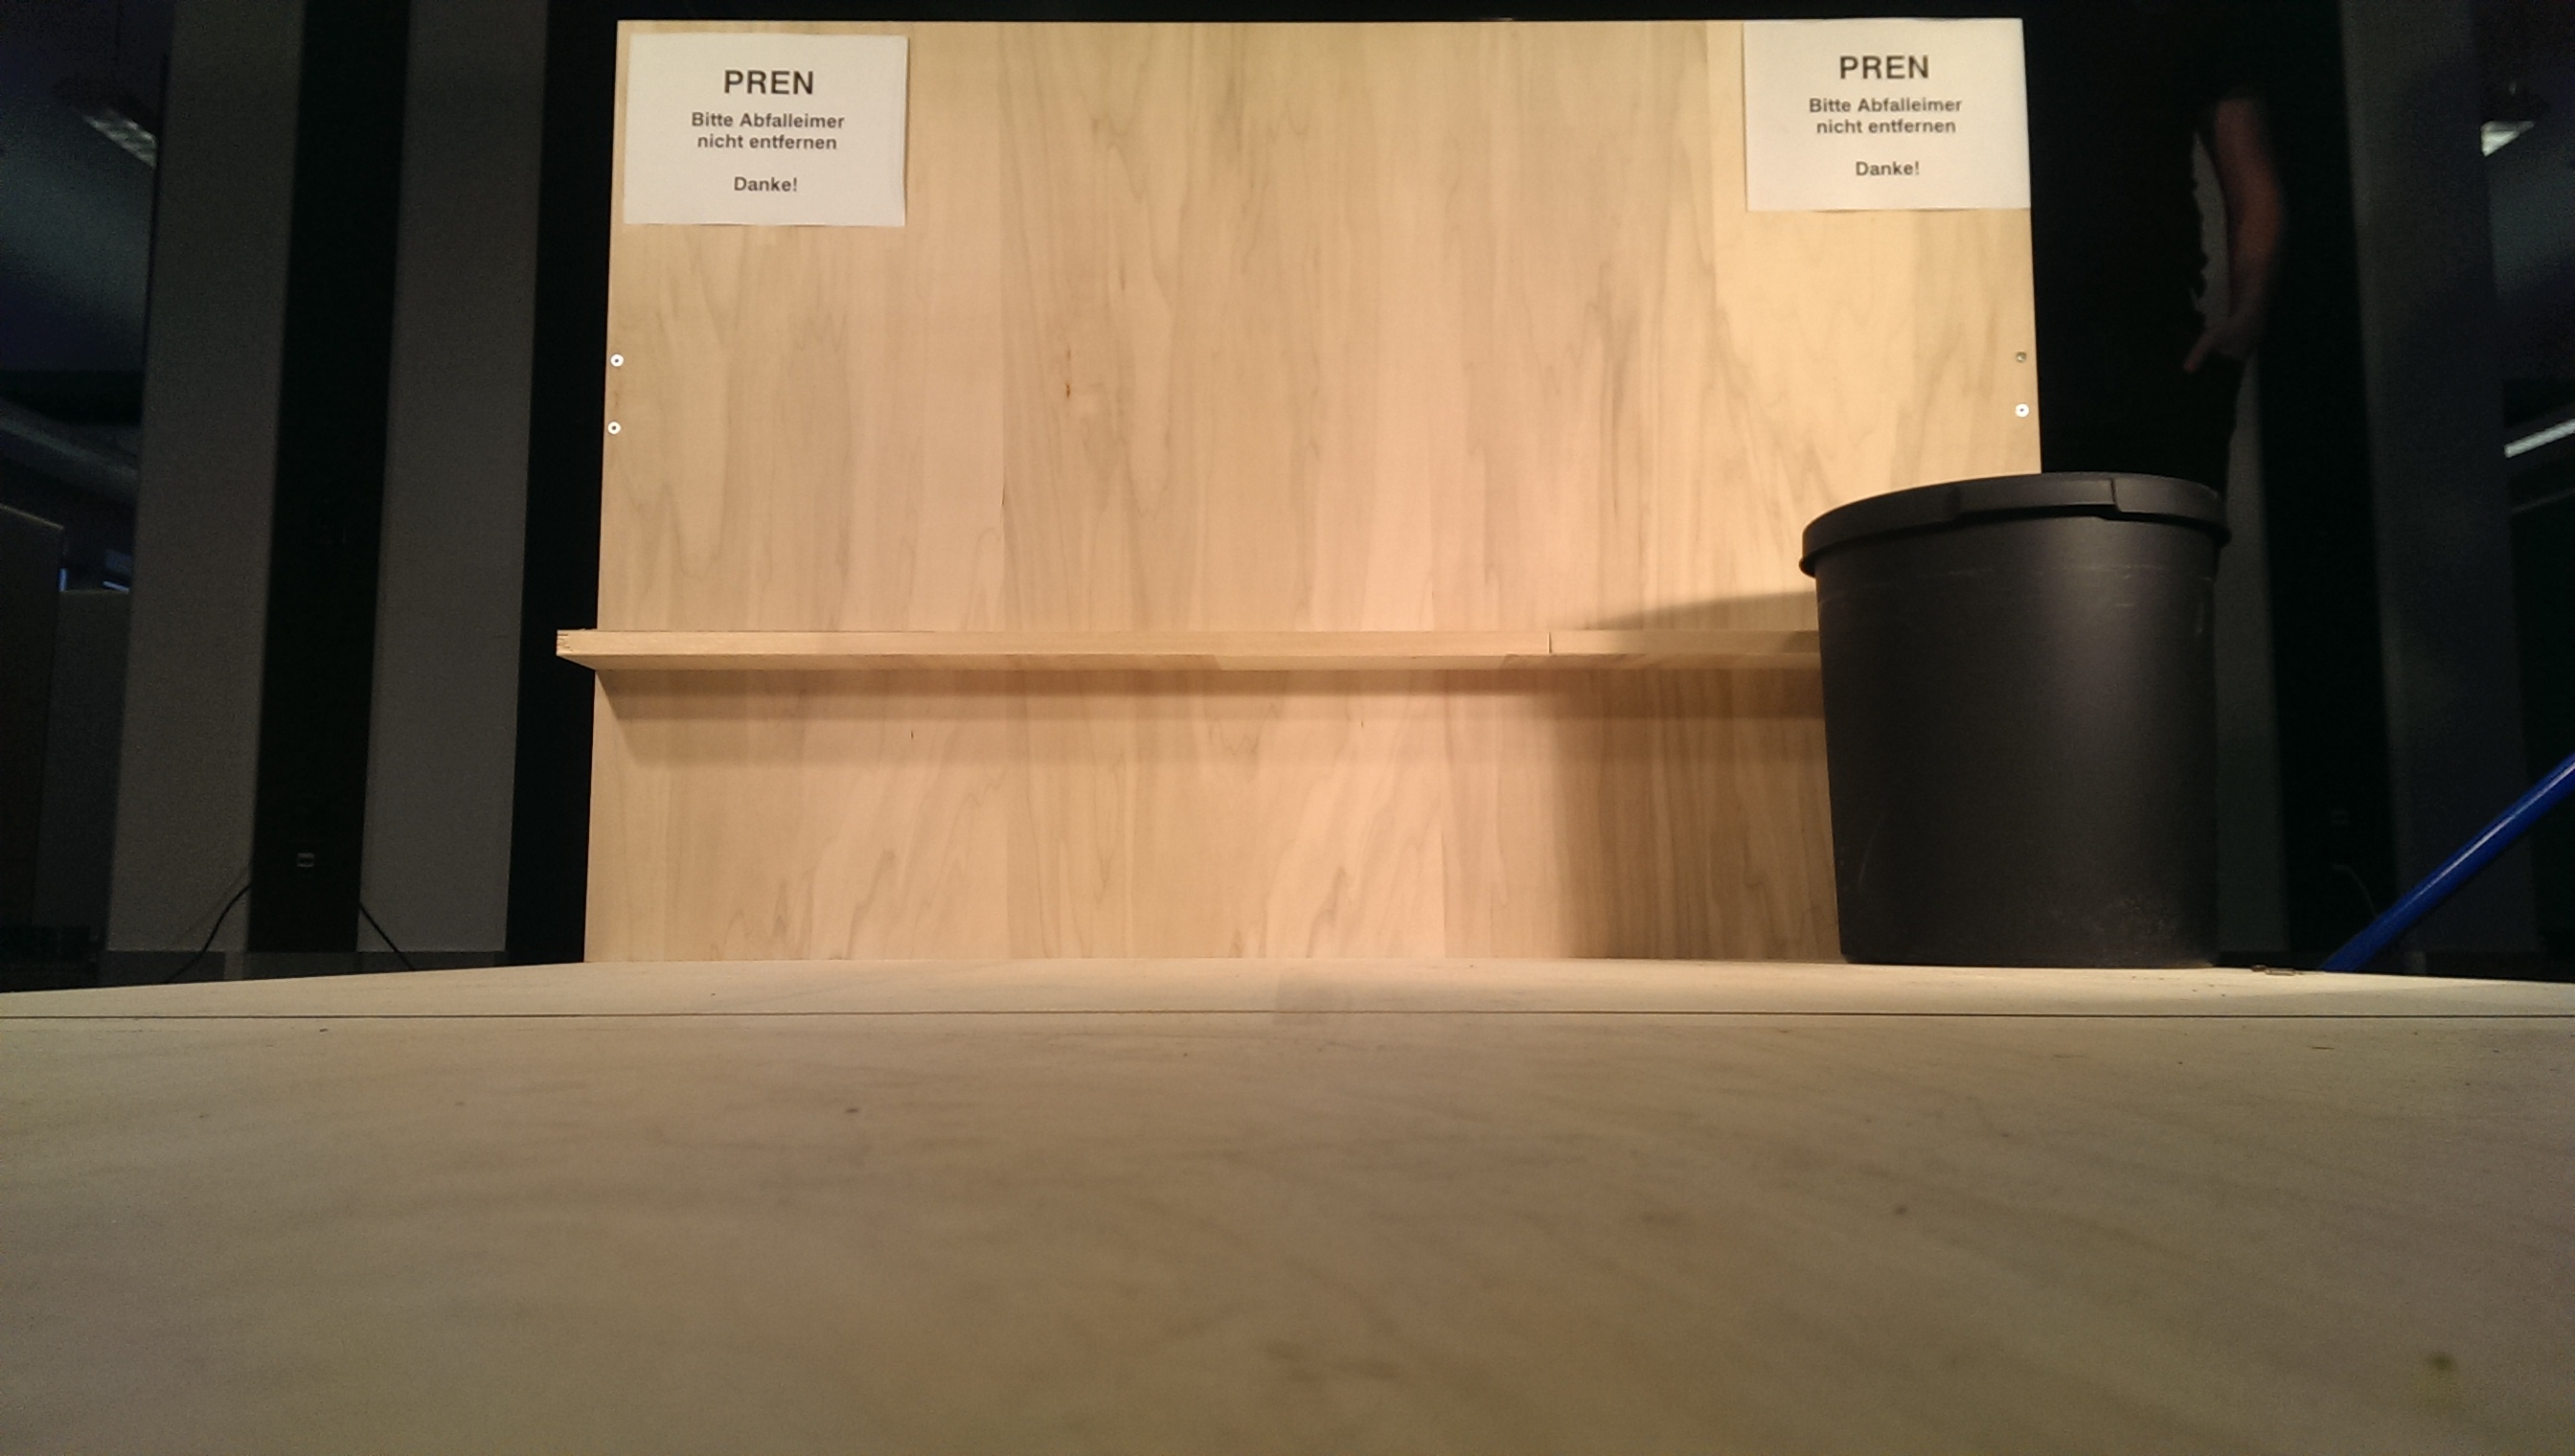
\includegraphics[width=0.495\textwidth,clip,trim=55cm 14cm 10cm 11.4cm]
{Enddokumentation/Tests/Bilder/KorbRechts_HTC.jpg}}\hfill
\subfigure[Foto eines LG-Nexus]{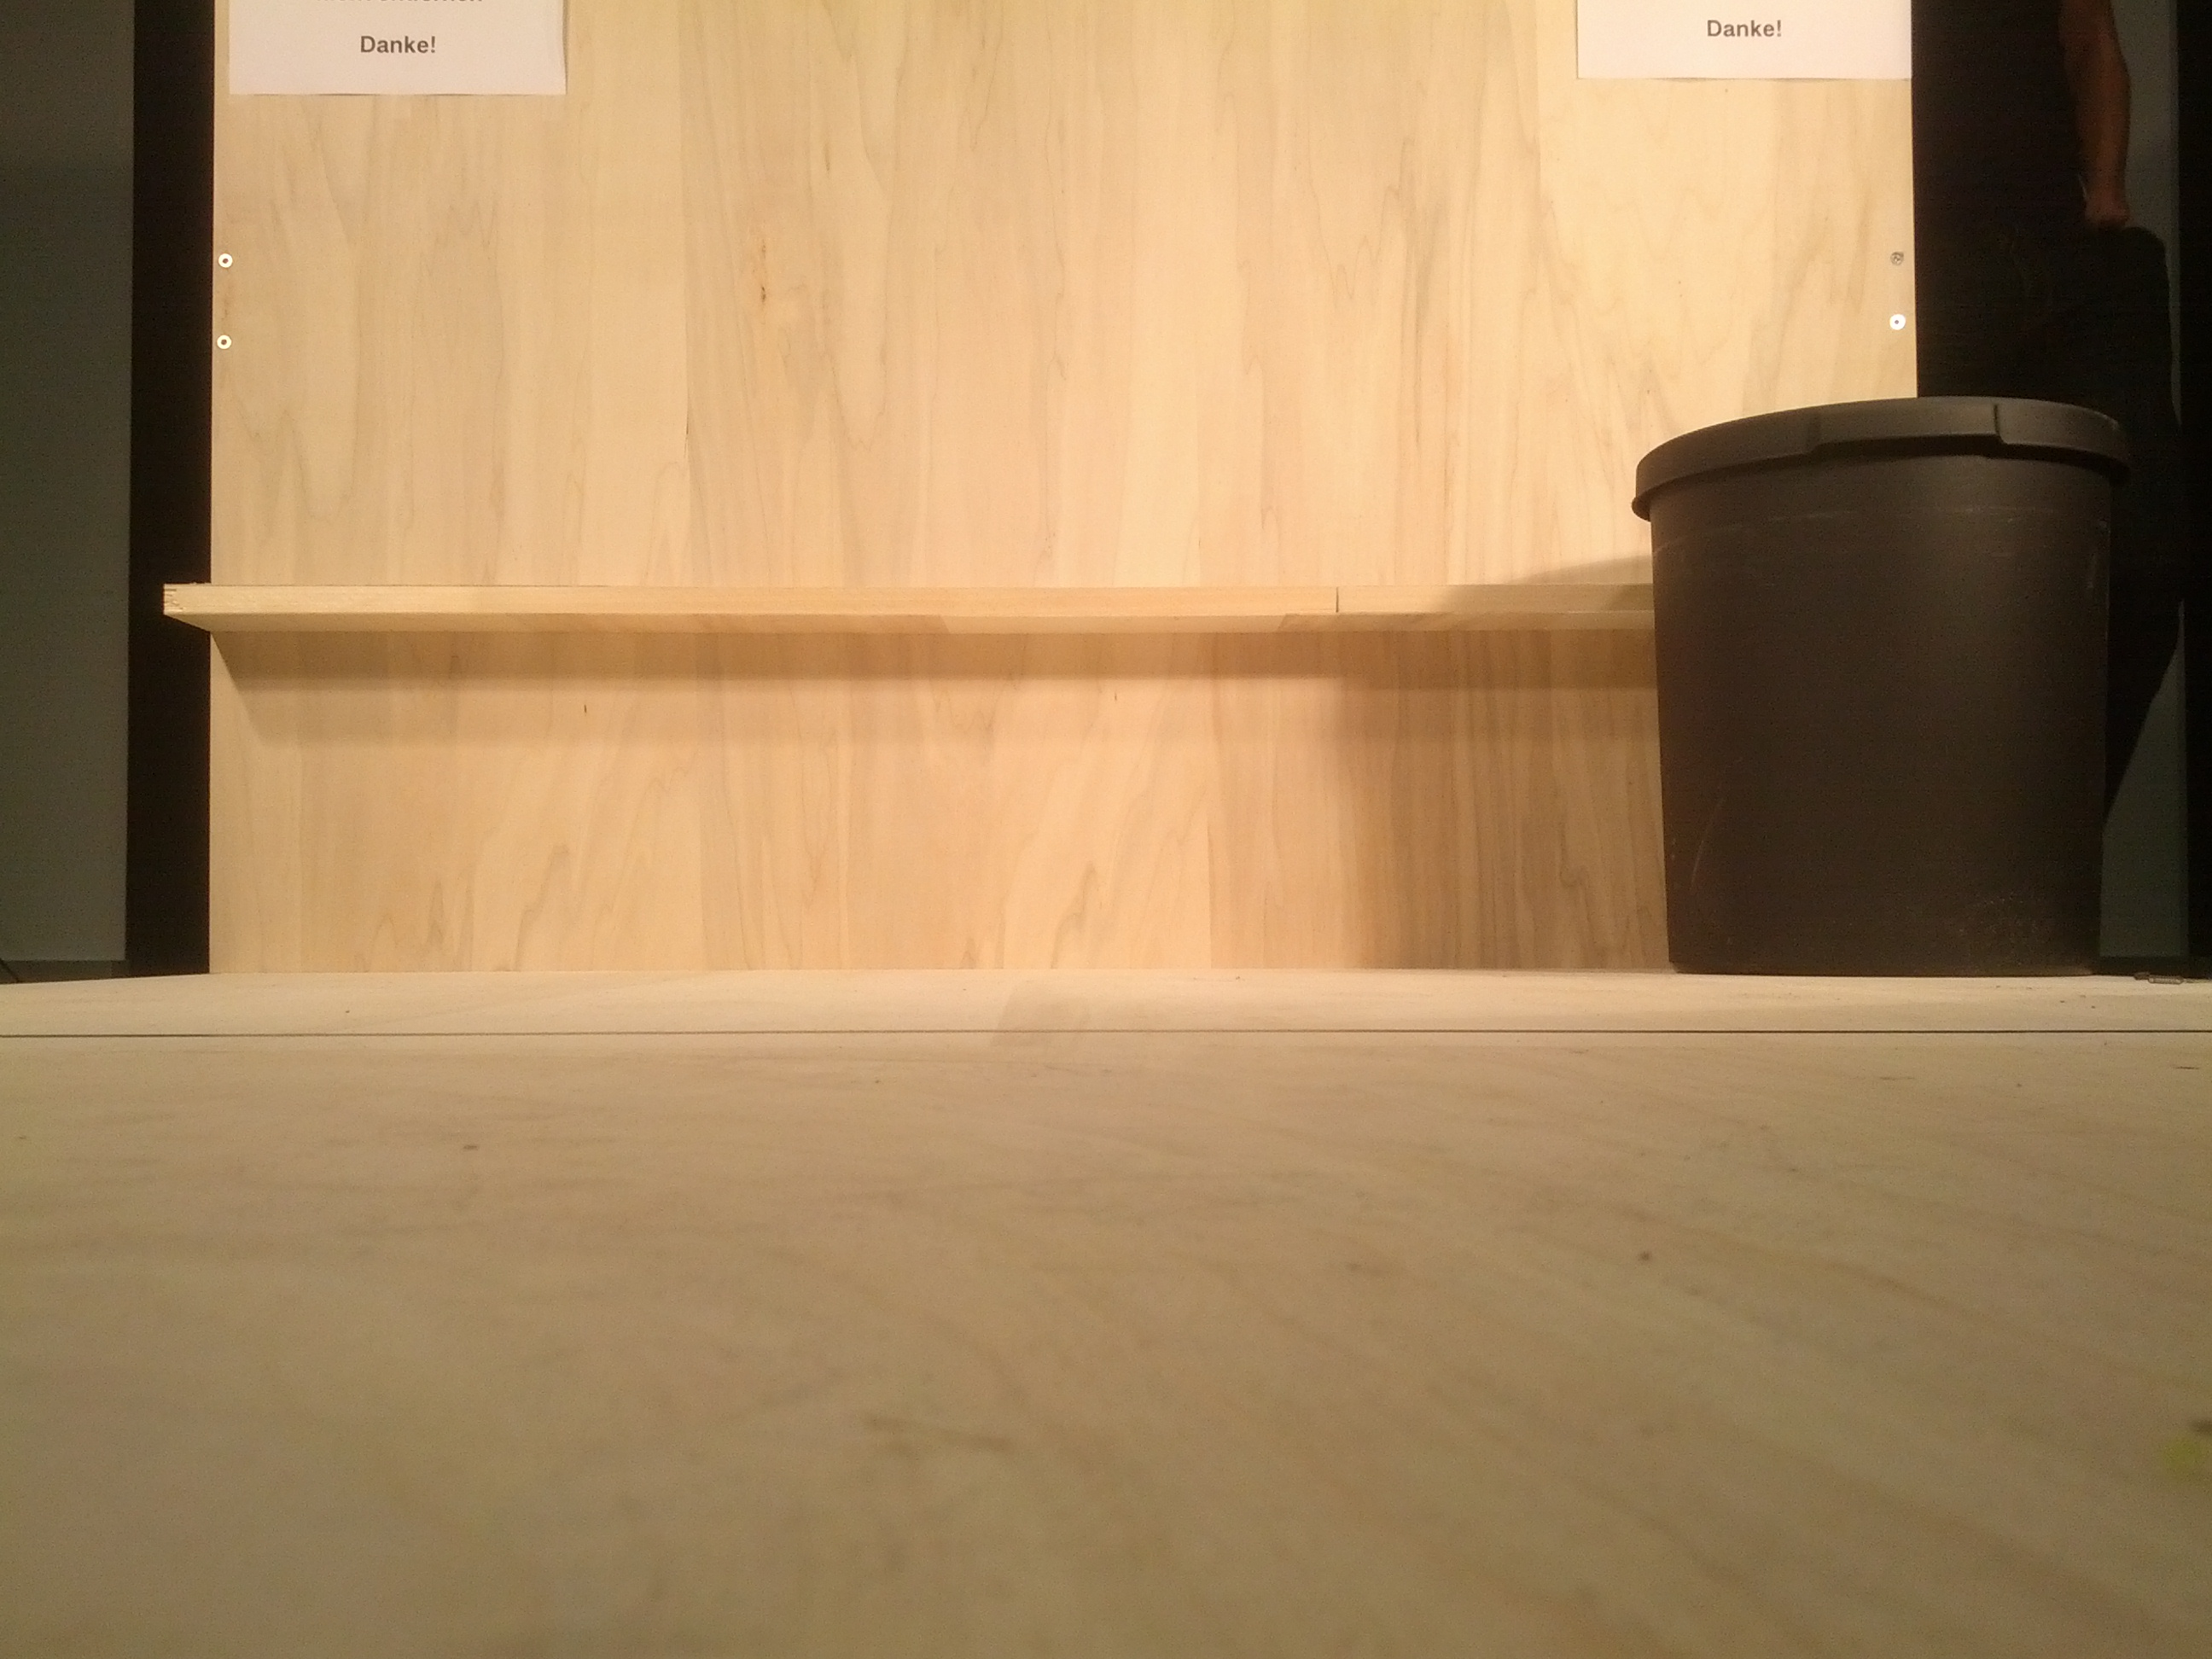
\includegraphics[width=0.495\textwidth,clip,trim=54cm 20cm 2cm 15cm]
{Enddokumentation/Tests/Bilder/KorbRechts_Nexus.jpg}}
\caption{Fotos des Korbes, der am Rand steht}
\label{fig:KorbFoto1}
\end{figure}

In der Abbildung~\ref{fig:KorbFoto1} ist gut zu erkennen, wie der Schatten des Korbes auf die 
Rückwand geworfen wird. Da der Korb am rechten Rand steht, ist nur der Schatten auf der linken 
von belang. Auch gut ersichtlich ist, dass der Kontrast dennoch ausreicht, um die Kontur des Korbes zu definieren.
\newpage
%
\begin{figure}[h!]
\subfigure[Foto eines HTC One]{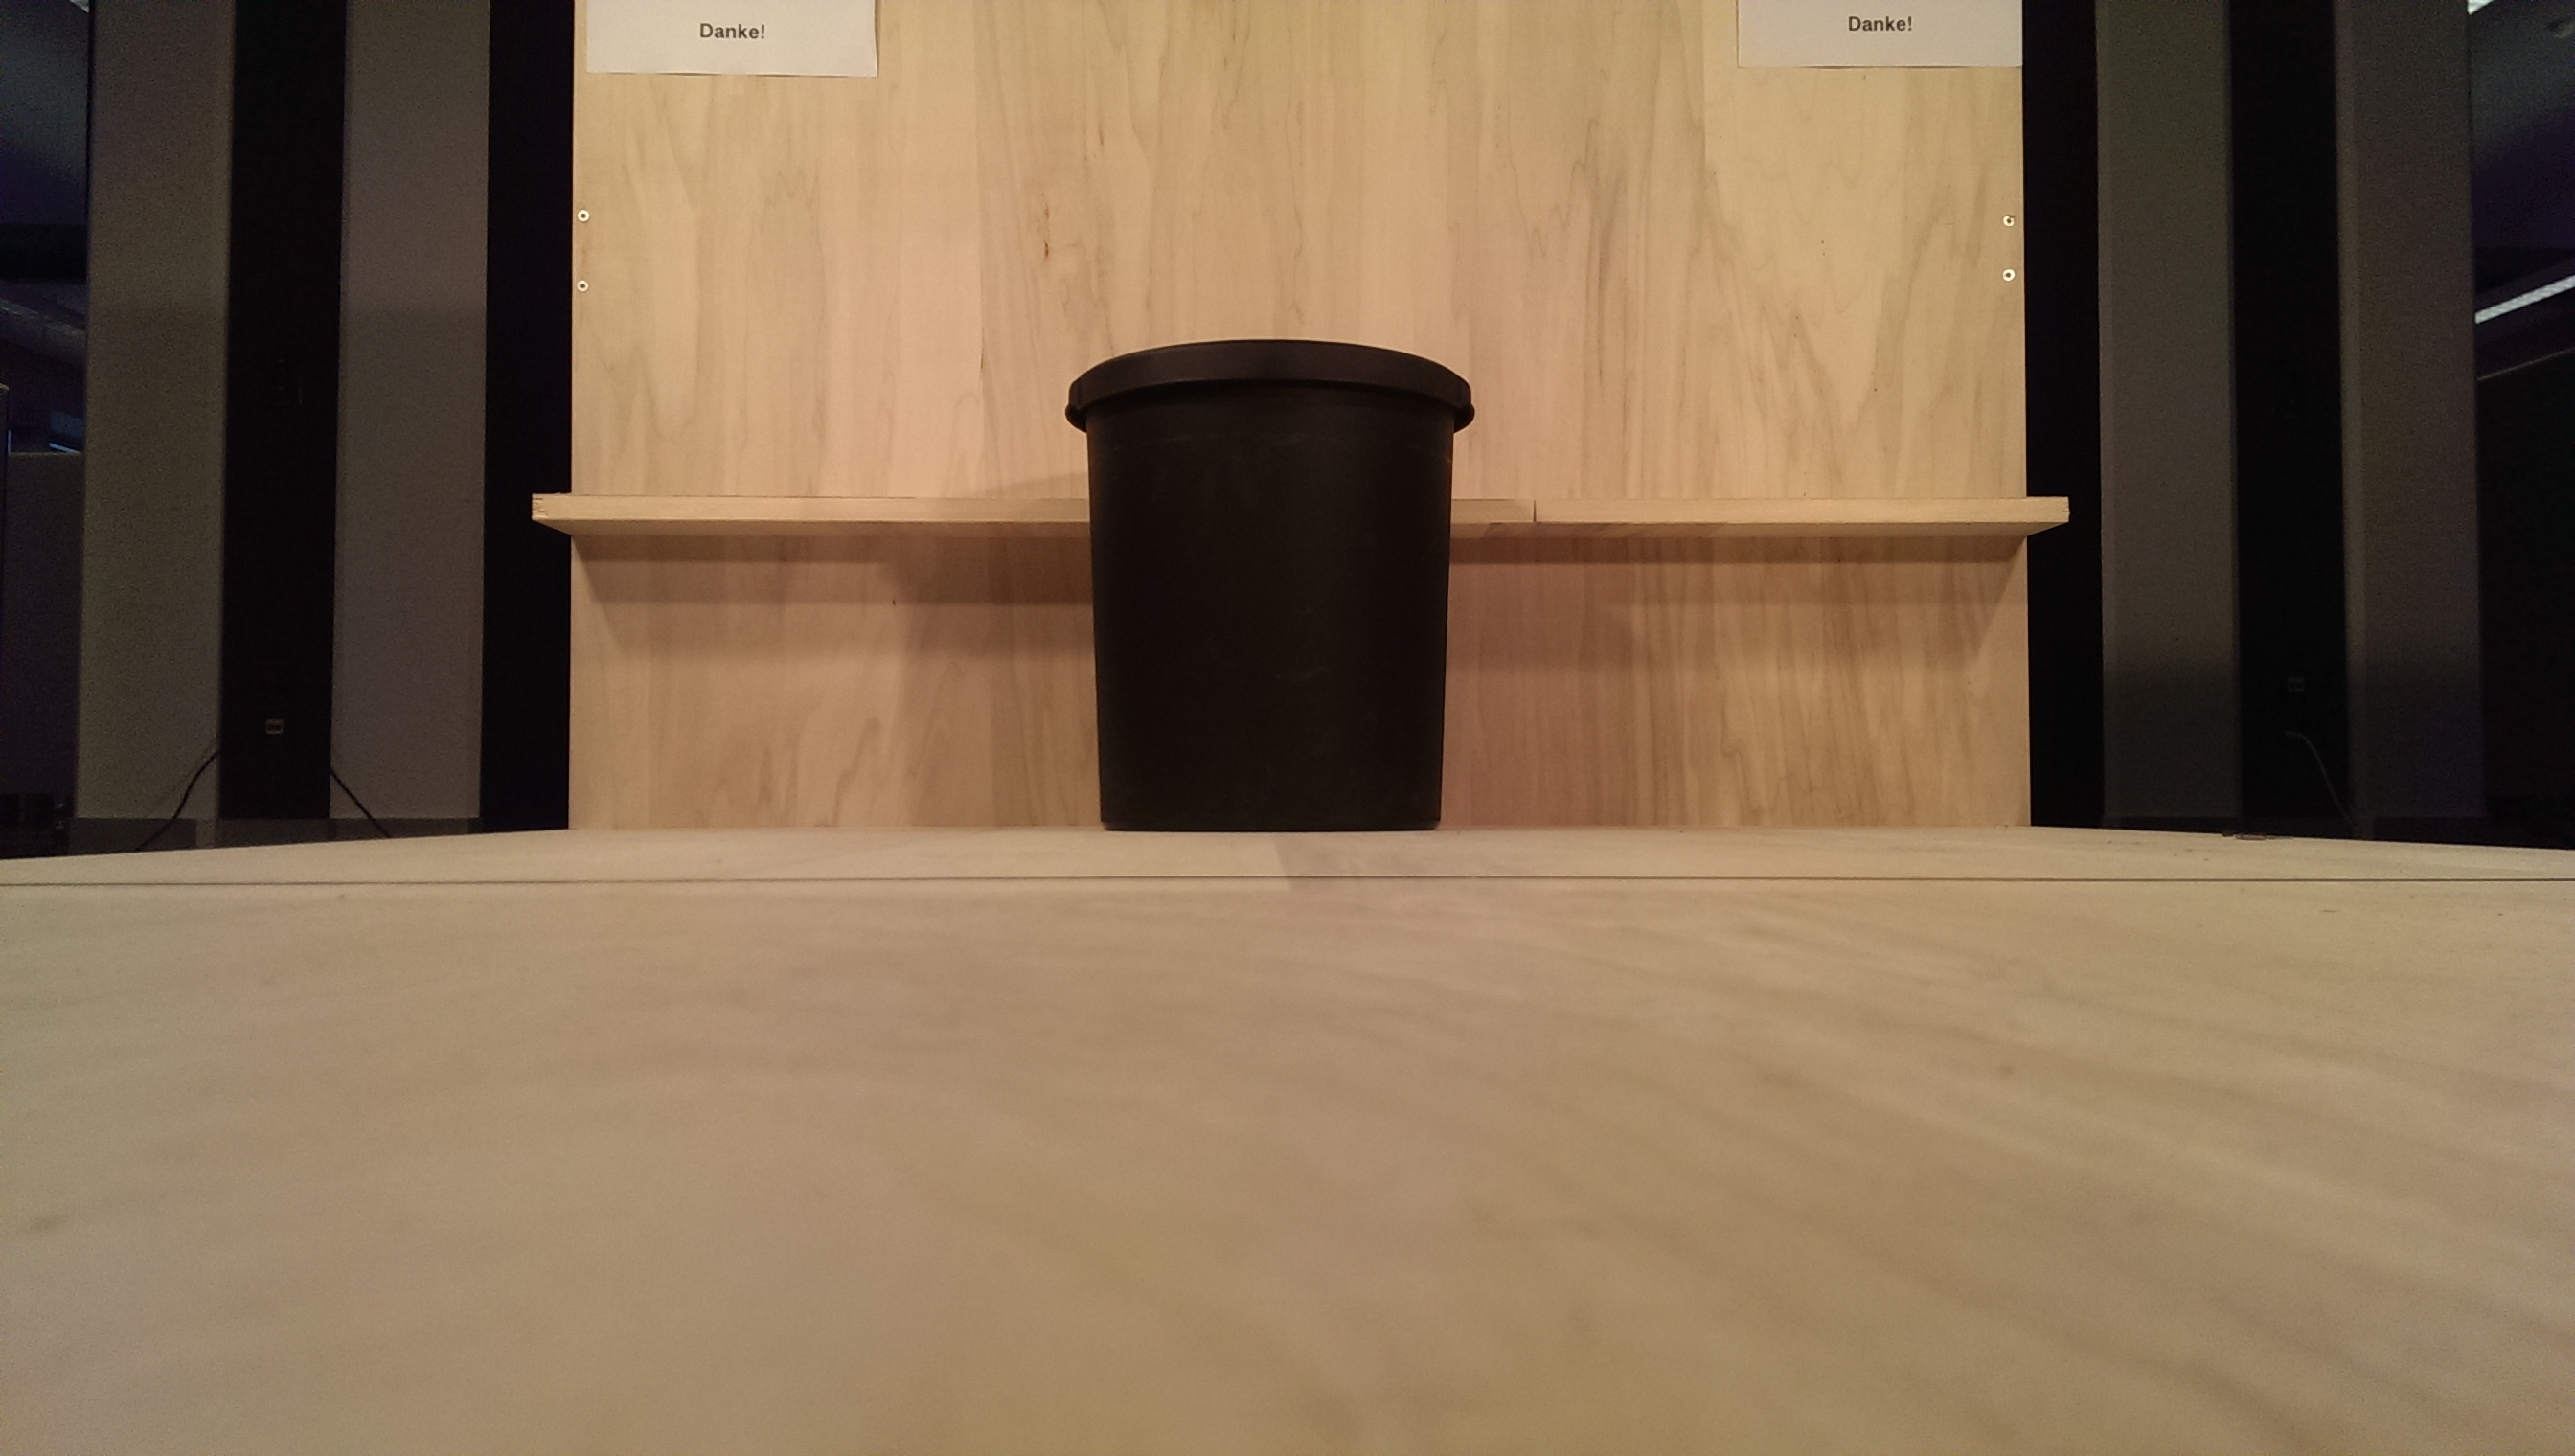
\includegraphics[width=0.495\textwidth,clip,trim=30cm 17cm 30cm 7cm]
{Enddokumentation/Tests/Bilder/KorbMitte_HTC.jpg}}\hfill
\subfigure[Foto eines LG-Nexus]{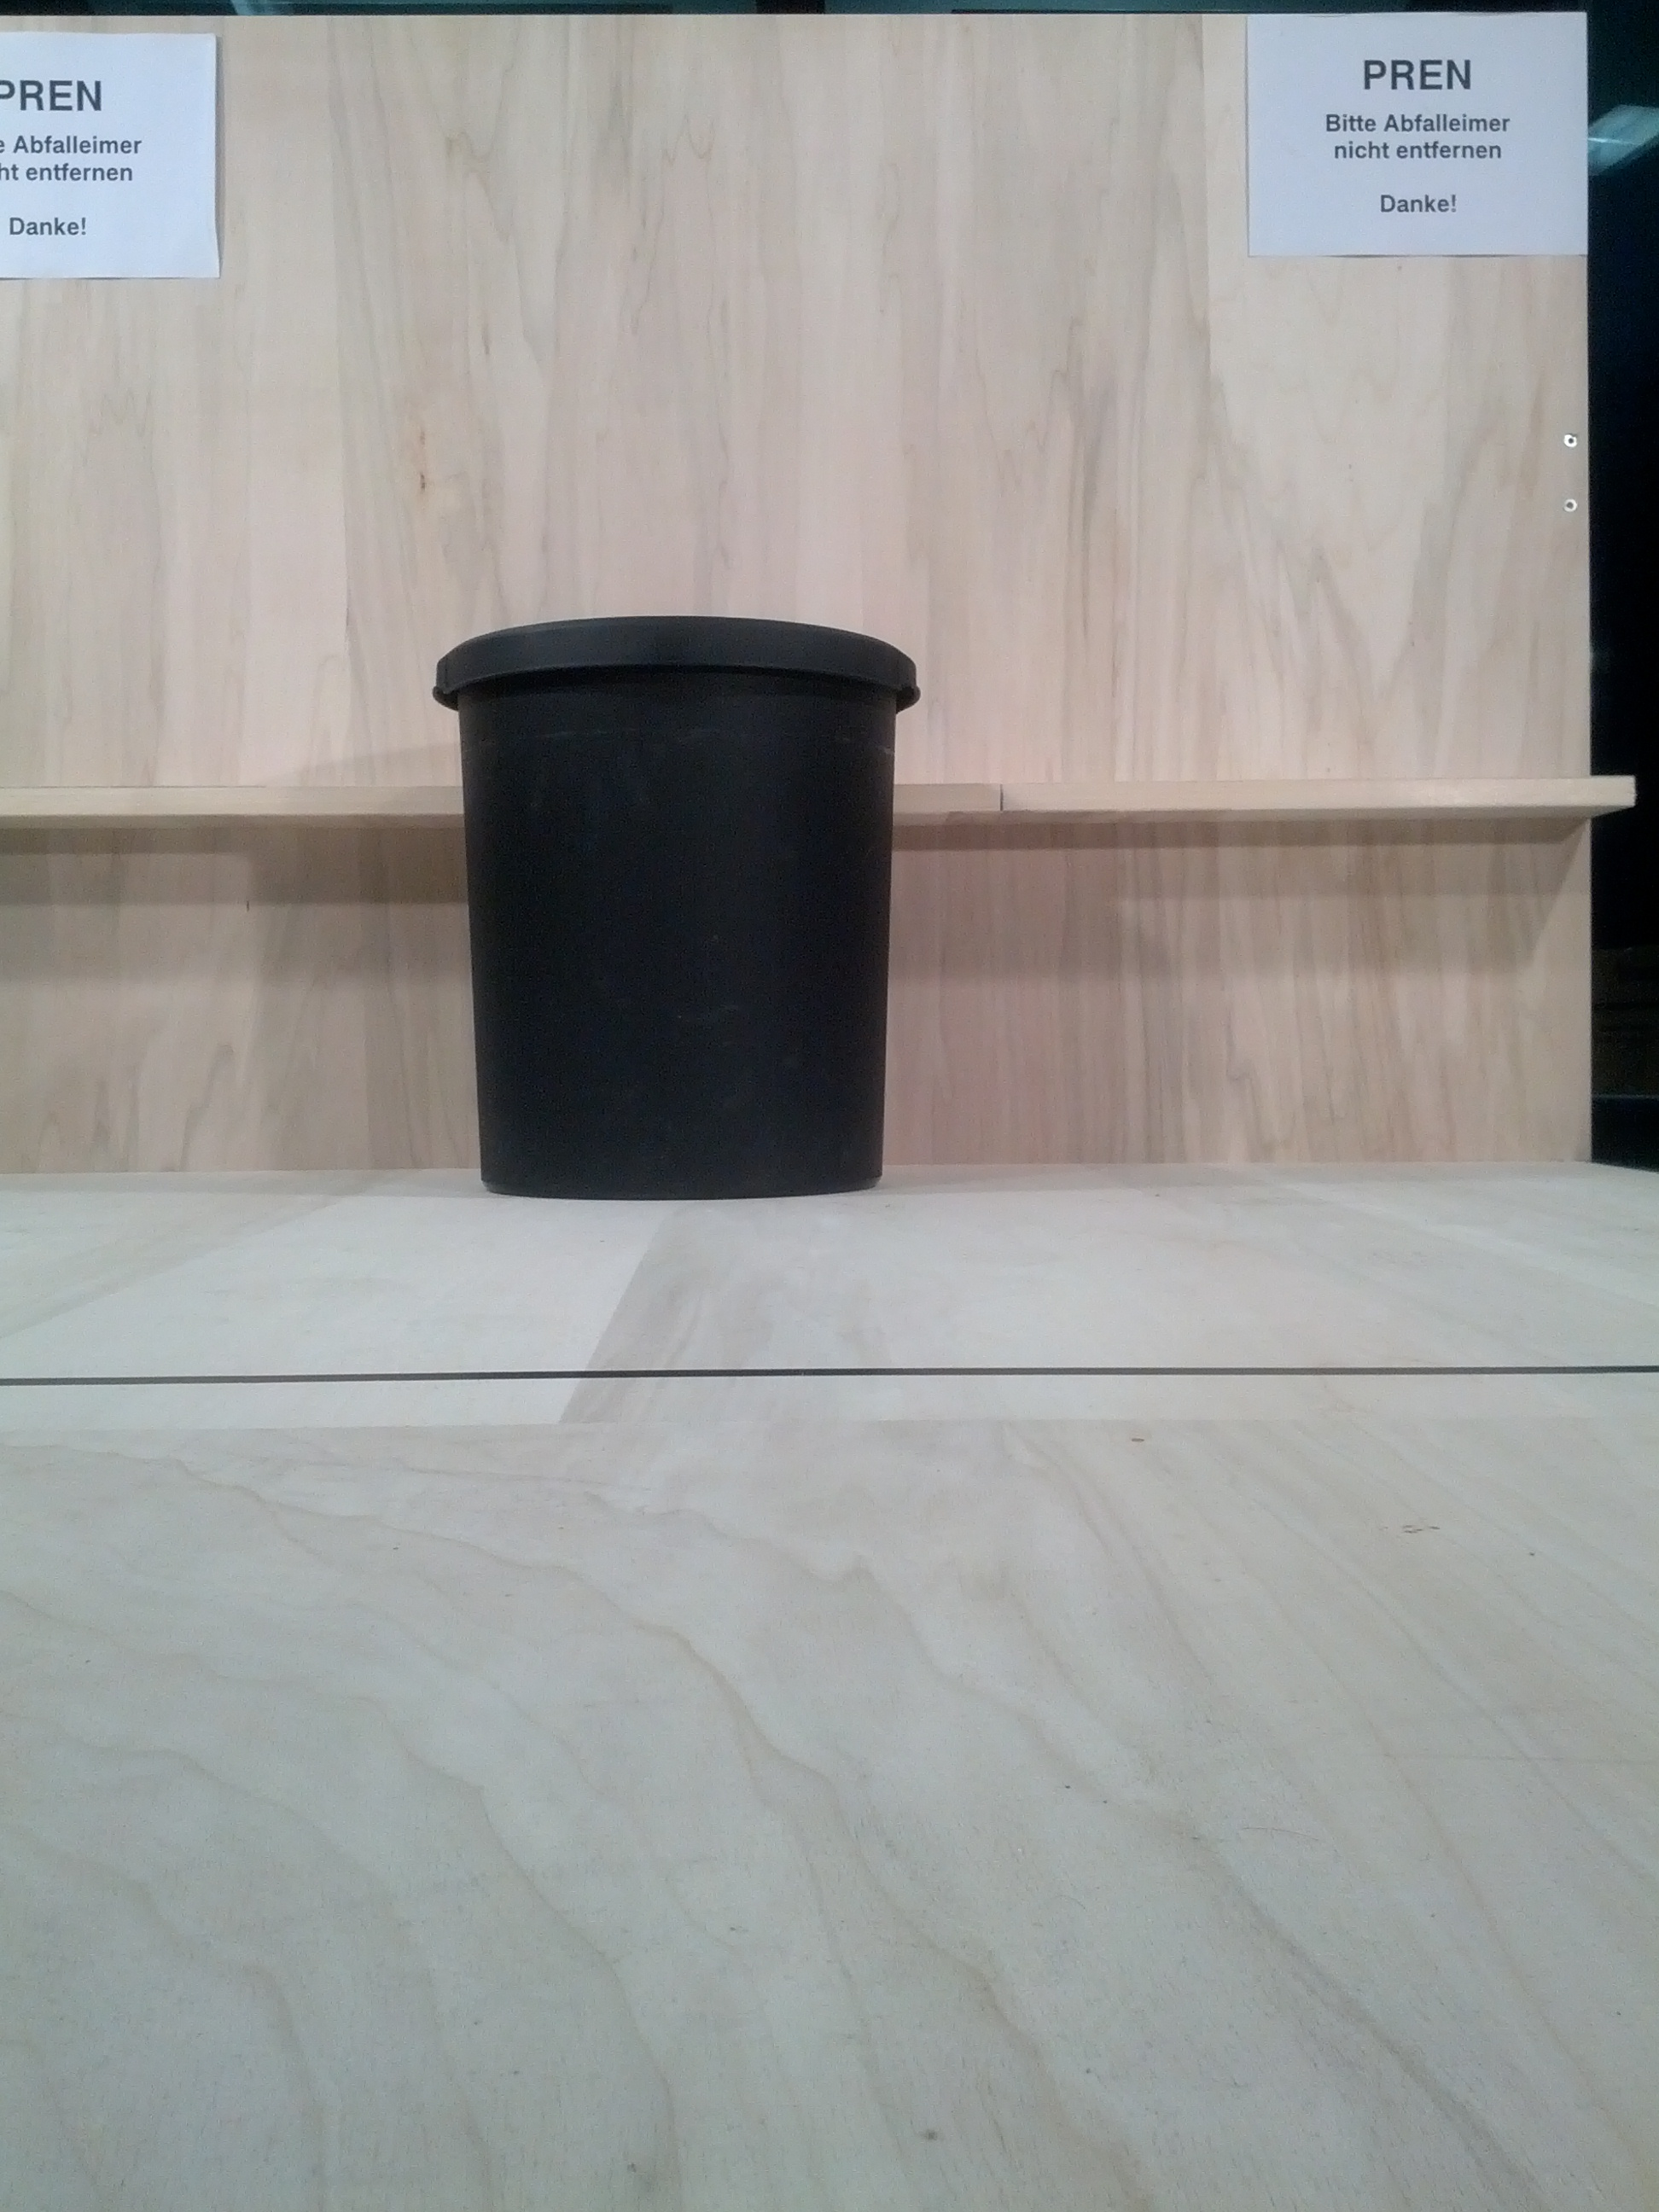
\includegraphics[width=0.495\textwidth,clip,trim=5cm 35.7cm 18cm 17cm]
{Enddokumentation/Tests/Bilder/KorbMitte_Nexus.jpg}}
\caption{Fotos des Korbes, der in der Mitte steht}
\label{fig:KorbFoto2}
\end{figure}
In der Abbildung~\ref{fig:KorbFoto2} ist zu erkennen, wie die Schatten des Korbes auf beide Seiten der Rückwand geworfen werden, deren Ausprägung jedoch deutlich geringer wie in Abbildung~\ref{fig:KorbFoto1} ist.






